\documentclass[10pt,sans,english,compress,xcolor=dvipsnames]{beamer}
\author[Lily ]{ Dr Lily Asquith (Lily, she/her)}

\usetheme{Szeged}
%\defbeamertemplateparent{enumerate items}{enumerate item,enumerate subitem,enumerate subsubitem,enumerate mini template}
\definecolor{titcol}{RGB}{16,78,100} 
\setbeamercolor{frametitle}{fg=titcol,bg=White}
\useoutertheme{miniframes} 
\useinnertheme{rectangles}

\usepackage{pifont}
\newcommand{\tick}{\textcolor{grn}{\ding{52} } }
\newcommand{\nope}{\textcolor{red}{\ding{54} } }


\usepackage{soul}
\usepackage{cancel}

\usepackage[most]{tcolorbox}
\definecolor{LilyBlack}{rgb}{0.05,0.1,0.3} % UBC Blue (primary)
\usecolortheme[named=LilyBlack]{structure}

\usepackage{booktabs}
\usepackage{tabularx}
%\usepackage{tikz}
%\def\checkmark{\tikz\fill[scale=0.4](0,.35) -- (.25,0) -- (1,.7) -- (.25,.15) -- cycle;}

\usepackage{physics}

\usepackage{xparse}

\setbeamertemplate{footline}{%
  \leavevmode%
  \hbox{\begin{beamercolorbox}[wd=.5\paperwidth,ht=2.5ex,dp=1.125ex,leftskip=.3cm plus1fill,rightskip=.3cm]{author in head/foot}%
    \usebeamerfont{author in head/foot}\insertshortauthor
  \end{beamercolorbox}%
  \begin{beamercolorbox}[wd=.5\paperwidth,ht=2.5ex,dp=1.125ex,leftskip=.3cm,rightskip=.3cm plus1fil]{title in head/foot}%
    \usebeamerfont{title in head/foot}\insertshorttitle\hfill\insertframenumber\,/\,\inserttotalframenumber
  \end{beamercolorbox}}%
  \vskip0pt%
}

\DeclareMathSizes{10}{10}{6}{4} % this one
%\DeclareMathSizes{10.95}{10}{6}{4}   % For size 10 text

\newcommand*\ColorBox[3][black]{%
  \makebox[2em][c]{%
    \setlength\fboxsep{-.5\fboxrule}%
    \raisebox{\dimexpr-#3em+.5ex}{%
      \fcolorbox{#1}{#2}{%
        \rule{0pt}{\dimexpr#3em*2}%
        \rule{\dimexpr#3em*2}{0pt}%
      }%
    }%
  }%
}

\usepackage{hyperref}
\hypersetup{
    colorlinks=true,
    linkcolor=blue,
    filecolor=magenta,      
    urlcolor=blue,
    pdftitle={Overleaf Example},
    pdfpagemode=FullScreen,
    }

\urlstyle{same}

% this part excludes specified frames from counters in navigation bar
\makeatletter
\let\beamer@writeslidentry@miniframeson=\beamer@writeslidentry
\def\beamer@writeslidentry@miniframesoff{%
  \expandafter\beamer@ifempty\expandafter{\beamer@framestartpage}{}% does not happen normally
  {%else
    % removed \addtocontents commands
    \clearpage\beamer@notesactions%
  }
}
\newcommand*{\miniframeson}{\let\beamer@writeslidentry=\beamer@writeslidentry@miniframeson}
\newcommand*{\miniframesoff}{\let\beamer@writeslidentry=\beamer@writeslidentry@miniframesoff}
\makeatother


\makeatletter
\newcommand\notsotiny{\@setfontsize\notsotiny{6.5}{7.5}}
\makeatother




\usepackage{multicol}
\usepackage{sansmath}
\usepackage{minted}
\definecolor{LightGray}{gray}{0.95}
\usepackage{nicematrix}
%\usepackage{statmath}
\usepackage{cancel}
\newcommand<>{\xxcancel}[1]{\alt#2{ \textcolor{red}{\cancel{#1}}\vphantom{#1} }{#1}}
\usepackage{tikz}

\usepackage{array}
\newcolumntype{L}{>{$}l<{$}}


\title[Least Squares]{Least Squares}
\date{}
\titlegraphic{
%\center

\includegraphics[scale=0.15]{sussex-logo}
}
% Lily includes for font and spacing
\usepackage{cmbright} % pretty nice but maybe a bit too different
\renewcommand{\baselinestretch}{1.1} 
\usepackage{sansmath}
% Lily highlight numerical answers for quicker marking
\usepackage{xcolor}
\definecolor{mygreen}{RGB}{226,254,226}
\definecolor{mylblue}{RGB}{205, 248, 250}
\definecolor{mylpink}{RGB}{159, 43, 104}
\usepackage[most]{tcolorbox}

\newtcbox[auto counter]{\ghl}
{enhanced, on line, boxsep=0pt,left=6pt,right=6pt,top=2pt,bottom=2pt,rightrule=1pt,
colback=mygreen,
colframe=black 
}
\newtcbox[auto counter]{\bhl}
{enhanced, on line, boxsep=0pt,left=6pt,right=6pt,top=2pt,bottom=2pt,rightrule=1pt,
colback=mylblue,
colframe=black 
}
\newtcbox[auto counter]{\yhl}
{enhanced, on line, boxsep=0pt,left=2pt,right=2pt,top=1pt,bottom=1pt,rightrule=1pt,
colback=lyellow,
colframe=black 
}

\newcommand{\bhlm}[1]{\bhl{$#1$}}

\newtcbox[auto counter]{\phl}
{enhanced, on line, boxsep=0pt,left=6pt,right=6pt,top=2pt,bottom=2pt,rightrule=1pt,
colback=mylpink,
colframe=black 
}

\DeclareMathOperator*{\plim}{plim}
\begin{document}

\newcommand\info{\mathcal{J}_{\theta}}
\newcommand\loglike{\ln{ \mathcal{L}_{\theta}} }
\newcommand\like{\mathcal{L}_{\theta} }

\newcommand\thetahat{\hat{ \theta }  }

\definecolor{grn}{RGB}{0,128,0} 
\newcommand{\gbl}[1]{\textcolor{grn}{#1}}

\definecolor{wh}{rgb}{0.95, 0.95, 0.96}
\newcommand{\wht}[1]{\textcolor{wh}{#1}}

%\newcommand{\inprob}{\overset{p}{\to}}

\newcommand{\boo}[1]{\textbf{\textcolor{red}{#1}}}

\newcommand{\covmat}{\mathbf{\textcolor{magenta}{\Sigma}} }


\definecolor{purr}{RGB}{128,0,128} 
\newcommand{\purp}[1]{\textcolor{purr}{#1}}

\newcommand{\magt}[1]{\textbf{\textcolor{magenta}{#1}}}
 \newcommand{\magtn}[1]{\textcolor{magenta}{#1}}
 
%\definecolor{bbl}{RGB}{128,0,128} 
\newcommand{\bbl}[1]{\textcolor{blue}{#1}}

\newcommand{\rbl}[1]{\textcolor{red}{#1}}

\definecolor{dblu}{RGB}{37,150,190} 
\newcommand{\blu}[1]{\textcolor{dblu}{#1} }

\definecolor{dor}{RGB}{255,40,0} 
\newcommand{\dor}[1]{\textcolor{dor}{#1} }

\definecolor{darkgreen}{RGB}{46,139,87} 
\newcommand{\dgreen}[1]{\textbf{\textcolor{darkgreen}{#1}} }
%\newcommand{\gbl}[1]{\textcolor{darkgreen}{#1}}

\definecolor{lgray}{RGB}{222,222,222} 

\definecolor{lyellow}{RGB}{255,255,224} 

\newcommand{\E}[1]{\mathbf{E}_{#1}}
%
\newcommand{\rvX}[1]{X_{(#1)} } 

\newcommand{\rvY}[1]{Y_{(#1)} }

\newcommand{\rvx}[1]{x_{(#1)} } 

\newcommand{\rvy}[1]{y_{(#1)} }



\newcommand{\red}[1]{\textcolor{red}{#1} }

\newcommand{\bluedots}{\blu{\ldots} }

\newcommand{\dordots}{\dor{\ldots} }


\newcommand{\where}{\dgreen{\;where\;} }


\newcommand{\pand}{\dgreen{\;and\;} }
\newcommand{\por}{\dgreen{\;or\;} }

\newcommand{\sumN}{ \sum\limits_{\blu{i}}^{\blu{N}} }

\newcommand{\sumZ}{ \sum\limits_{\dor{j}}^{\dor{Z}} }

\newcommand{\Expec}[1]{ \mathbb{E}[#1] }


\newcommand{\Xfj}[1]{ X_{ \dor{#1} } }

\newcommand{\xfi}[1]{ x_{ \blu{#1} } }

\newcommand{\Xij}[2]{ X_{\mage{#1},\blu{#2} }}

\newcommand{\sumxi}{ \sumN \xfi{i} }

\newcommand{\sumXj}{ \sumZ \Xfj{j} }

\newcommand{\sumZa}[1]{ \sumZ {#1}_{ \dor{j} } }

\newcommand{\sumZab}[2]{ \sumZ {#1}_{ \dor{j} }\, {#2}_{ \dor{j} } }

\newcommand{\sumNab}[2]{ \sumN {#1}_{ \blu{i} }\, {#2}_{ \blu{i} } }

\newcommand{\vecxi }{ [ \xfi{1} \xfi{2}, \bluedots, \xfi{N} ] }

\newcommand{\vecXj }{ [ \Xfj{1} \Xfj{2}, \bluedots, \Xfj{Z} ] }

\newcommand{\vecXij }{ [ \Xij{1}{1} \Xij{1}{2}, \bluedots, \Xij{1}{N_1} ],\, [ \Xij{2}{1} \Xij{2}{2}, \bluedots, \Xij{2}{N_2} ],\, \dordots,\,[ \Xij{Z}{1} \Xij{Z}{2}, \bluedots, \Xij{Z}{N_Z} ] }

% definitions

\newcommand{\overNblack}{ \dfrac{1}{N} }
\newcommand{\overN}{ \dfrac{1}{ \blu{N} } }

\newcommand{\defmean }{ \overline{x} = \overN \sumN \xfi{i} }

\newcommand{\meanx }{ \overline{x} }
\newcommand{\meansqx }{ \overline{x^2} }
\newcommand{\sqmeanx }{ \overline{x}^2 }
\newcommand{\devsq}{ (\xfi{i} - \meanx)^2 }

%\newcommand{\var }[1]{ \mathcal{V}_{#1} }
\newcommand{\defvar }{ \var{x} = \overN \sumN \devsq }
\newcommand{\defvarshort }{ \var{x} = \meansqx - \sqmeanx }

\newcommand{\defstd }{ s_x = \sqrt{ \var{x} }  }

\newcommand{\defwmean }{ \overline{X} = \dfrac{ \sumZab{w}{X} }{ \sumZa{w} } }  

\newcommand{\defw }{ w_{\dor{j}} = \dfrac{1}{ \var{\Xfj{j} } } }



\begin{frame}
\titlepage
\end{frame} 

\section*{Preamble}


\begin{frame}{MEQ}

\begin{center}

\includegraphics[scale=0.35]{MEQ-2025.png}
\end{center}

\end{frame} 



% contents
\begin{frame}{Least Squares, Tests}
\small
\begin{itemize}
\item Today: \magtn{Least Squares}: the math behind that call to \texttt{fit}.
\end{itemize}
\begin{itemize}
\item Wednesday: \bbl{Test Statistics} (Z, T, F/ ANOVA, LR, AIC, BIC, $\chi^2$)
\end{itemize}

\vspace{1cm}

This slide deck is only for Least Squares. I'm afraid the times when my lecture notes were up a week or two in advance are now soundly behind us... \\
%For these last weeks, I can only promise that lecture notes will be up before the lecture starts. \\

\end{frame} 

%\begin{frame}{Naive Bayes}
%\footnotesize
%
%MLE also used to train Neural Networks : loss function is often negloglike\\[1ex]
%Transformers
%Gaussian Mixture models, Hidden Markov models, also apparently use MLE.\\[1ex]
%
%
%\end{frame}


\begin{frame}{Intro, reminder of big picture}
\footnotesize

Fitting means estimating the parameters, and sometimes also the functional form, that best describes a dataset.\\[1ex]

A functional form can have one parameter or lots of them. \\[1ex]

The least squares approach minimises the residuals for all parameters simultaneously, to provide the best set of parameter estimates.\\[1ex]

The math is a bit cumbersome, but I have done my best to keep it clean and clear. \\[1ex]

\end{frame} 






\begin{frame}{Least Squares}
\footnotesize
%\magtn{Least} \bbl{Squares} $\equiv$ \magtn{Minimise} \bbl{Squared Residuals}\\[1ex]




\begin{center}
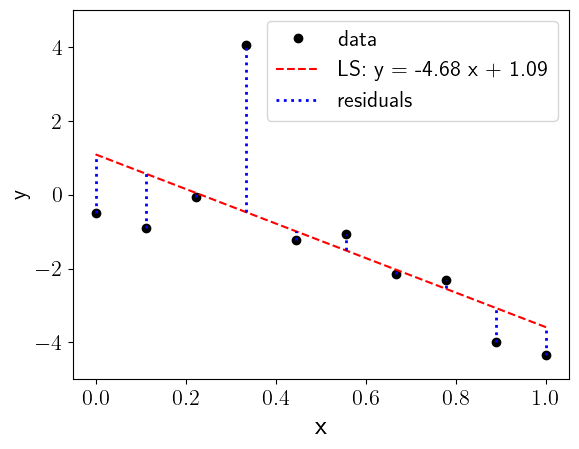
\includegraphics[scale=0.4]{LinearLeastSquaresExample_c1.0_m-5.2_noise2.4_outliers2.png}
\end{center}


The Least Squares \rbl{fit} is a simultaneous estimation of the parameters of the function $y(x)$. The estimates are found by taking the derivatives of the sum of the squared \bbl{residuals} ($\chi^2$) and setting them to zero.\\[1ex]


\end{frame} 



\begin{frame}{Chi Squared}
\footnotesize
Pearson's Chi Squared, $\chi^2$, is  the sum of the squared \magtn{standardised} \bbl{residuals}:\\
\begin{center}
\bhl{$\chi^2 = \sum\limits_i^N \dfrac{ (\bbl{y_i - \mu})^2}{\magtn{\sigma^2_i}} $} \\[1ex]
\end{center}
\vspace{0.2cm}

$y_i$ is the measurement of  the RV $Y$.\\[1ex]
$\mu$ is the True Value of $y_i$.\\[1ex]
$\sigma_i$ is the standard deviation of a normal distribution centred on the true value $\mu$ .\\[1ex]

The numerator is the uncertainty in the model, aka the Residual Sum of Squares (RSS),\\[1ex]

%, aka the Unexplained Variance\bbl{*}).

 The denominator is the uncertainty in the data, aka the Total Sum of Squares (TSS).\\[1ex]
 
 %\bbl{* The Explained Variance is denominator-numerator.}\\

\end{frame} 


\begin{frame}{Why Chi Squared? \hfill \footnotesize \bhl{$\chi^2 = \sum\limits_i^N \dfrac{ (\bbl{y_i - \mu})^2}{\magtn{\sigma^2_i}} $}
}
\footnotesize
Last week we wrote the Log Likelihood for Gaussian as:\\[1ex]
\yhl{$ \loglike = - N \ln{ \sigma} - N \ln{ \sqrt{2\pi}} - \dfrac{1}{2} \sum\limits_i^N \dfrac{(y_i-\mu)^2}{\sigma^2}$}\\[1ex]

This assumes that $\sigma$ is the same for every measurement $y_i$, or in other words that the $y_i$ are from the same Gaussian distribution with true parameter $\sigma$.\\[1ex]

 If we avoid that assumption (\bbl{homoscedasticity}) we find:\\[1ex]
\ghl{$\loglike = -\sum\limits_i^N \ln{ \sigma_i} - N \ln{ \sqrt{2\pi}} - \dfrac{1}{2} \sum\limits_i^N \dfrac{(y_i-\mu)^2}{\sigma_i^2}$}\\[2ex]

Note that we no longer have two parameters to estimate, but $N+1$! \magtn{Oops...}\\


\end{frame} 


\begin{frame}{Why Chi Squared? \hfill \footnotesize \bhl{$\chi^2 = \sum\limits_i^N \dfrac{ (\bbl{y_i - \mu})^2}{\magtn{\sigma^2_i}} $}
}
\footnotesize
It's okay. All the $\sigma_i$ estimates will have the same form:\\

$\dfrac{\partial}{\partial \sigma_i}\ln\mathcal{L}_{\sigma_i} = - \sum\limits_i^N\dfrac{1}{\sigma_i} - 0 + \sum\limits_i^N \dfrac{(y_i-\mu)^2}{\sigma_i^3} =0$\;\;\\[1ex]

 \bbl{therefore}\;\;$\sum\limits_i^N \dfrac{(y_i-\mu)^2}{\sigma^3}  = \sum\limits_i^N \dfrac{1}{\sigma}$\;\;\; \bbl{when}\;\;\; $ \sum\limits_i^N \sigma_i^2 = \sum\limits_i^N (y_i-\mu)^2 $\\[1ex] 
 
 The best estimate for all $\sigma_i$ is that which results in $\chi^2 = \sum\limits_i^N \dfrac{ (\bbl{y_i - \mu})^2}{\magtn{\sigma^2_i}}  = 0$.\\[1ex]
 
 This is also the case for the best estimate for $\mu$. \magtn{Minimising $\chi^2$ is exactly equivalent to finding the MLE for $\mu$ and (all of the) $\sigma$.}
\end{frame} 





\begin{frame}{Chi Squared with Binned Data\hfill \footnotesize \bhl{$\chi^2 = \sum\limits_i^N \dfrac{ (\bbl{y_i - \mu})^2}{\magtn{\sigma^2_i}} $}}
\footnotesize

In real life we bin our measurements using histograms. We count the number of measurements in a small range of $\Delta y$ (the bin width) and the height of the histogram bar is the number of measurements that fall in that interval.\\[1ex]

In this case, we adjust our definition: \ghl{$\chi^2 = \sum\limits_i^N \dfrac{ (n_i -\mu)^2 }{n_i} = \sum\limits_i^N \dfrac{(obs -exp)^2}{obs}$}\\[1ex]

The use of $n_i$ in place of $\sigma_i^2$ is correct because in the binned case we are using bin counts, which means we are using \magtn{Poisson statistics}. \\[1ex]

The Poisson RV is a rate (a \magtn{count}, in a given time), $E[K]=\lambda$, and the variance is $V[K] = \lambda$. For fixed time, the rate is a count, and the squared uncertainty $V[K] = \sigma^2$ is $\lambda \equiv n$.

\end{frame} 


\section*{$y=mx+c$}

\begin{frame}{The Equation of a Straight Line}
\footnotesize
A straight line in the $x,y$ plane is described by \ghl{$y = mx +c$}, where $m$ is the slope and $c$ is the intercept on the $y$-axis.\\[1ex]

The control variable is $x$ and the RV is $y$: the thing we are measuring.\\[1ex]

\magtn{Example}:\\
Every hour, I measure my heart rate. Time is the control variable $x$, with evenly spaced intervals and negligible uncertainty. My measured heart rate is $y$, a random variable,  with uncertainty.\\[1ex]

If my heart rate increases steadily throughout the day from 70 to 100 beats per minute over a period of 10 hours, then $m = 30/10 =3$ and $c = 70$. \ghl{$y = 3x + 70$}.\\[1ex]



\end{frame} 


\begin{frame}{Constructing the $\chi^2$ \hfill \footnotesize \bhl{$y = mx +c$}}
\footnotesize
$\chi^2 = \sum\limits_i^N \dfrac{ (y_i - \bbl{\hat{\mu}})^2}{\sigma^2_i} $\magtn{\;\;True $\mu$ is estimated from the fit: $\hat{\mu}$.} \\[1ex]

A straight line fit of the form $\hat{\mu} = \hat{m}x_i+\hat{c}$ provides $\hat{m}$ and $\hat{c}$: the parameter estimates that minimise $\chi^2$. The Estimate for $Y$ is the expected value of our measurement,  \bbl{$\hat{\mu}= E[y_i]$}.\\[1ex]

$\chi^2 = \sum\limits_i^N \dfrac{ (y_i - \bbl{(mx_i +c)} )^2}{\sigma^2_i} $ \\[1ex]

%The numerator:  $( y_i - \bbl{mx_i}  - \bbl{c} )^2  = y^2_i + \bbl{m^2x^2_i}  + \bbl{c^2}  + \bbl{2cmx_i} - \bbl{2c}y_i - \bbl{2mx_i}y_i $\\

$\chi^2 = \sum\limits_i^N \dfrac{1}{\sigma_i^2} \left(y^2_i + m^2x^2_i  + c^2  + 2cmx_i - 2cy_i - 2mx_iy_i\right)$\\[1ex]

\end{frame} 


\begin{frame}{Derivatives of \hfill \footnotesize{$\chi^2 = \sum\limits_i^N \dfrac{1}{\sigma_i^2} \left(y^2_i + m^2x^2_i  + c^2  + 2cmx_i - 2cy_i - 2mx_iy_i\right)$} }
\footnotesize
\magtn{As with the MLE}, we find the parameters that minimise $\chi^2$ by taking the first derivative with respect to each one.\\[1ex]

We will put the \bbl{second derivatives} in our pocket for later, when we calculate the uncertainties.\\[2ex]

%$\chi^2 = \sum\limits_i^N \dfrac{1}{\sigma_i^2} \left(y^2_i + m^2x^2_i  + c^2  + 2cmx_i - 2cy_i - 2mx_iy_i\right)$\\[3ex]

$\magtn{ \dfrac{\partial \chi^2}{\partial m} }
= \sum\limits_i^N
\dfrac{1}{\sigma_i^2}
( 2\,m\,x^2_i + 2\,c\,x_i - 2\, x_i\,y_i )$\hspace{2cm}\bbl{$\dfrac{\partial^2 \chi^2}{\partial m^2} 
= \sum\limits_i^N
\dfrac{1}{\sigma_i^2}
( 2\,x^2_i )$}\\[2ex]


$\magtn{\dfrac{\partial \chi^2}{\partial c} }
= \sum\limits_i^N
\dfrac{1}{\sigma_i^2}
( 2\,c +  2\,m\,x_i - 2\,y_i)$\hspace{2.6cm}\bbl{$\dfrac{\partial^2 \chi^2}{\partial c^2} 
= \sum\limits_i^N
\dfrac{1}{\sigma_i^2}
( 2)$}\\[2ex]

\hspace{6.9cm}\bbl{$\dfrac{\partial^2 \chi^2}{\partial c \partial m}  = \sum\limits_i^N \dfrac{1}{\sigma_i^2} ( 2x_i)$}\\[2ex]

\end{frame} 


\begin{frame}{Two parameter estimation }
\footnotesize
\magtn{As with the MLE}, we estimate the parameters by setting the partial derivatives to zero and solving for $m$ and $c$, which gives us:\\[1ex]

$\sum\limits_i^N
\dfrac{1}{\sigma_i^2}y_ix_i  = 
\sum\limits_i^N\dfrac{1}{\sigma_i^2}( mx^2_i+ cx_i  )$\\[3ex]

$\sum\limits_i^N
\dfrac{1}{\sigma_i^2}y_i = 
\sum\limits_i^N\dfrac{1}{\sigma_i^2}( mx_i+ c  )$\\[3ex]

We have found ourselves with two simultaneous equations (we have two parameters) and we need to solve them.  

\end{frame} 

\begin{frame}{Shorthand}
\footnotesize
Sums and squared sigmas are common everywhere, so we can \magtn{tidy things up with shorthand}:\\[1ex]

$\bbl{s_1} = \sum\limits_i^N \dfrac{1}{\sigma^2_i}$\;\;\;\;\; $\bbl{s_x} = \sum\limits_i^N \dfrac{x_i}{\sigma^2_i}$\;\;\;\;\;$\bbl{s_{xx}} = \sum\limits_i^N \dfrac{x^2_i}{\sigma^2_i}$\;\;\;\;\;$\bbl{s_y} = \sum\limits_i^N \dfrac{y_i}{\sigma^2_i}$\;\;\;\;\;$\bbl{s_{xy}} = \sum\limits_i^N \dfrac{x_i y_i}{\sigma^2_i}$\\[1ex]

We have:\\[1ex]

$\sum\limits_i^N
\dfrac{1}{\sigma_i^2}y_ix_i  = 
\sum\limits_i^N\dfrac{1}{\sigma_i^2}( mx^2_i+ cx_i  )$\;\;\;\ding{234}\;\;\; \bbl{$s_{xy} =  s_{xx}\, m +  s_{x}\, c$}\\[3ex]

$\sum\limits_i^N
\dfrac{1}{\sigma_i^2}y_i = 
\sum\limits_i^N\dfrac{1}{\sigma_i^2}( mx_i+ c  )$\;\;\;\;\;\;\;\;\;\;\ding{234}\;\;\; \bbl{$s_y = s_x\, m +  s_1\,c$}\\[3ex]


\end{frame} 



\begin{frame}{Solving simultaneous equations for $m$ and $c$}
\footnotesize
We have:\\[1ex]
 $ s_{xx}\, \bbl{m} +  s_{x}\, \rbl{c} = s_{xy} $\hspace{1cm}[\magt{1}]\\[1ex]
$  s_x\, \bbl{m} +  s_1\,\rbl{c}  = s_y $\hspace{1.2cm}[\magt{2}]\\[1ex]

Eliminate \bbl{$m$} by multiplying through and subtracting:\\[1ex]
$s_{xx} [\magt{2}] - s_x [\magt{1}] $:\hspace{0.5cm}$(s_{xx} s_1 - s_x s_x )\,\rbl{c} = s_{xx} s_y - s_x s_{xy} $\;\;\; \bhl{$\rbl{c} = \dfrac{ \rbl{s_{xx} s_y - s_x s_{xy} }  }{ s_{xx} s_1 - s_x s_x}$ }\\[1ex]

Eliminate \rbl{$c$} by multiplying through and subtracting:\\[1ex]
$ s_1 [\magt{1}] - s_{x} [\magt{2}] $:\hspace{0.5cm}$(  s_1 s_{xx} - s_{x} s_x )\,\bbl{m} =    s_1 s_{xy} - s_{x} s_y$\;\;\;\bhl{$\bbl{m} = \dfrac{  \bbl{s_1 s_{xy} - s_{x} s_y }  }{  s_1 s_{xx} - s_{x} s_x}$ }\\[1ex]

Note the denominator is \bhl{$s_1 s_{xx} - s_{x} s_x =\Delta$}: independent of $y$.

\end{frame} 




\begin{frame}{Solving with Cramer's Method}
\footnotesize
A 'shortcut' to solving for $m$ and $c$ is to use Cramer's Method: we construct matrices of pairs of coefficients and take their determinants.\\[1ex]
 $ s_{xx}\, \bbl{m} +  s_{x}\, \rbl{c} = s_{xy} $\hspace{1cm}[\magt{1}]\\[1ex]
$  s_x\, \bbl{m} +  s_1\,\rbl{c}  = s_y $\hspace{1.2cm}[\magt{2}]\\[1ex]

The coefficients of m and c: $\begin{vmatrix}
  s_{xx} & s_{x}  \\
s_x&  s_1   \\
\end{vmatrix}=
 s_{xx}s_1 - s_x s_x   = \Delta$\\[1ex]

The coefficients of m and 1: $\textcolor{red}{c=
\begin{vmatrix}
s_{xx} & s_{xy} \\ 
s_x & s_{y}  \\
\end{vmatrix}}\bigg/ \Delta=
\textcolor{red}{(  s_{xx}s_{y} - s_{xy} s_{x}   ) }/  \Delta
$\\[1ex]

The coefficients of 1 and c:\; $\textcolor{blue}{m=
\begin{vmatrix}
s_{xy} & s_{x}  \\ 
s_y & s_{1}  \\
\end{vmatrix}}\bigg/ \Delta=
\textcolor{blue}{ (s_{xy}s_1 - s_{x}s_{y} ) }/  \Delta
$\\[1ex]

Note the result is exactly the same as by solving directly. I don't find Cramer's way quicker...
\end{frame} 


\begin{frame}{Solutions}
\footnotesize
The solutions for our two parameter estimates are:\\[1ex]

$\begin{bmatrix}
\textcolor{blue}{\hat{m}}\\\textcolor{red}{\hat{c}}
\end{bmatrix}
= \dfrac{1}{\Delta}
\begin{bmatrix}
\textcolor{blue}{
  s_{xy}s_1 - s_{x}s_{y} }\\
\textcolor{red}{
 s_{xx} s_{y} -  s_{xy}s_{x} 
}
\end{bmatrix}$
\vspace{0.5cm}

Where we have used the shorthand notation:\\[1ex]

$s_1 = \sum\limits_i^N \dfrac{1}{\sigma^2_i}$\;\;\;\;\; $s_x = \sum\limits_i^N \dfrac{x_i}{\sigma^2_i}$\;\;\;\;\;$s_{xx} = \sum\limits_i^N \dfrac{x^2_i}{\sigma^2_i}$\;\;\;\;\;$s_y = \sum\limits_i^N \dfrac{y_i}{\sigma^2_i}$\;\;\;\;\;$s_{xy} = \sum\limits_i^N \dfrac{x_i y_i}{\sigma^2_i}$\\[1ex]

And $\Delta =  s_{xx}s_1 - s_x s_x$\\[1ex]
%\bbl{ $ s_{xx}\, m +  s_{x}\, c = s_{xy} $ }\\[1ex]
%\bbl{$  s_x\, m +  s_1\,c  = s_y$}\\[1ex]

\bbl{Note that without the shorthand notation we would be drowning in sums and squared sigmas. This is for the two parameters of a straight line with one independent variable.} 

\end{frame} 


\section*{Uncertainties}

\begin{frame}{Parameter Uncertainties}
\footnotesize
Now, how to get the uncertainties on these monstrous solutions for the parameters $m$ and $c$?\\[1ex]

 \magtn{Just as for the MLE}, we can use a Taylor expansion of $\chi^2$ about the estimated true parameter values:\\
\notsotiny
\begin{align*}
\chi^2(m,c)  &= \chi^2(\hat{m},\hat{c})\\[0.5ex]% \;\;\;\; \bbl{Minimum\;\chi^2}\\
& + \xxcancel{ \dfrac{\partial \chi^2}{\partial m}\bigg|_{\hat{m}}} \left(m-\hat{m}\right)
+ \xxcancel{ \dfrac{\partial \chi^2}{\partial c}\bigg|_{\hat{c}}} \left(c-\hat{c}\right) \hspace{2cm}\rbl{Zero\; by\; construction}\\[0.5ex]
& + \bbl{ \dfrac{1}{2!} \dfrac{\partial^2 \chi^2}{\partial m^2}\bigg|_{\hat{m}} }
\left(m-\hat{m}\right)^2
+ \bbl{\dfrac{1}{2!} \dfrac{\partial^2 \chi^2}{\partial c^2}\bigg|_{\hat{c}} }
\left(c-\hat{c}\right)^2 + \bbl{ 2\,\dfrac{1}{2!} \dfrac{\partial^2 \chi^2}{\partial m \partial c}\bigg|_{\hat{m},\hat{c} } }
\left(m-\hat{m}\right)\left(c-\hat{c}\right)\hspace{2cm}\\[0.5ex]
\end{align*}
\footnotesize
The \bbl{second order partial derivatives} are our Information terms. These are the elements of the Curvature Matrix.\\

\end{frame} 


\begin{frame}{Parameter Uncertainties}
\footnotesize
\magtn{The Hessian (or Curvature) Matrix is}:\\[1ex]

$
H = 
\begin{bmatrix}
\dfrac{1}{2!} \dfrac{\partial^2 \chi^2}{\partial m^2} &\dfrac{1}{2!} \dfrac{\partial^2 \chi^2}{\partial m \partial c}\\[3ex]
\dfrac{1}{2!} \dfrac{\partial^2 \chi^2}{\partial m \partial c}&\dfrac{1}{2!} \dfrac{\partial^2 \chi^2}{\partial c^2}
\end{bmatrix}
=
\bbl{
\begin{bmatrix}
s_{xx} &s_x\\[1ex]
s_x &s_1\\
\end{bmatrix}
}
$
\vspace{0.5cm}

Where we have obtained the \bbl{nice simplified form} using the shorthand for the second derivatives we calculated earlier:\\[1ex]


$\dfrac{\partial^2 \chi^2}{\partial m^2}  = \sum\limits_i^N \dfrac{1}{\sigma_i^2} ( 2x^2_i) = \bbl{2s_{xx}}$\hspace{1cm}$\dfrac{\partial^2 \chi^2}{\partial c^2}  = \sum\limits_i^N \dfrac{1}{\sigma_i^2} ( 2) = \bbl{2s_1}$\\[1ex]
$\dfrac{\partial^2 \chi^2}{\partial c \partial m}  = \sum\limits_i^N \dfrac{1}{\sigma_i^2} ( 2x_i) = \bbl{2s_x}$\\[1ex]


%Notice that the determinant of the Hessian, $|H|$ is our denominator $\Delta = s_{xx}s_1 - s_x s_x$\\[1ex]
\end{frame} 


\begin{frame}{Parameter Uncertainties}
\footnotesize
\begin{tikzpicture}[remember picture, overlay]
\node[xshift=-4cm,yshift=-1.7cm] at (current page.north east)
{
\notsotiny
\yhl{
Inverse of Matrix: $
\begin{bmatrix}
a & b\\
c & d
\end{bmatrix}^{-1} =
\dfrac{1}{
(ad-bc)}
\begin{bmatrix}
d & -c\\
-b & a
\end{bmatrix} 
$
}
};
\end{tikzpicture}


The \bbl{Inverse*} of the Hessian Matrix is the \magtn{Covariance Matrix} $\covmat = \bbl{\mathsf{H^{-1}}}$. \rbl{*}\\[1ex]

$
\mathsf{H} = 
\begin{bmatrix}
s_{xx} &s_x\\[1ex]
s_x &s_1\\
\end{bmatrix}
\hspace{1cm} \bbl{\mathsf{H^{-1}} = \dfrac{1}{s_{xx}s_1 -s_xs_x}
\begin{bmatrix}
s_{1} & -s_x\\[1ex]
- s_x &s_{xx}\\
\end{bmatrix}
= 
\dfrac{1}{\Delta}
\begin{bmatrix}
s_{1} & -s_x\\[1ex]
- s_x &s_{xx}\\
\end{bmatrix}}
$
\vspace{0.5cm}

$
\covmat \magtn{= 
\begin{bmatrix}
\sigma^2_m & cov(m,c)\\[1ex]
cov(m,c) &\sigma^2_c\\
\end{bmatrix}}
$
\vspace{0.5cm}

We find:\;\; \bhl{$\sigma_m^2 = \dfrac{s_1}{\Delta}$\;\;\;\;$\sigma_c^2 = \dfrac{s_{xx}}{\Delta}$\;\;\;\;$cov(m,c) = -\dfrac{s_x}{\Delta}$}\\[1ex]

The nonzero covariance terms tell us the parameters are correlated. If we change the gradient of the fit, $m$, we will change the intercept, $c$.\\[2ex]
\notsotiny
\rbl{* Recall the inverse of the Information was the minimum variance bound}
\end{frame} 



\begin{frame}{Matrix Notation}
\footnotesize
The Taylor expansion for $\chi^2$ about $\theta=\hat{\theta}$ is:\\[1ex]

\notsotiny
$\chi^2(m,c)  = \chi^2(\hat{m},\hat{c}) +\magtn{ \dfrac{1}{2!} \dfrac{\partial^2 \chi^2}{\partial m^2}\bigg|_{\hat{m}} } \bbl{ \left(m-\hat{m}\right)^2}
+ \magtn{ \dfrac{1}{2!} \dfrac{\partial^2 \chi^2}{\partial c^2}\bigg|_{\hat{c}} } \bbl{  \left(c-\hat{c}\right)^2} + \magtn{ 2\,\dfrac{1}{2!} \dfrac{\partial^2 \chi^2}{\partial m \partial c}\bigg|_{\hat{m},\hat{c} } } \bbl{ \left(m-\hat{m}\right)\left(c-\hat{c}\right)}$\\[2ex]
\vspace{0.5cm}

\footnotesize
In matrix notation this is:\\[1ex]
\notsotiny
$\chi^2(m,c) - \chi^2(\hat{m},\hat{c}) =
\bbl{
\begin{bmatrix}
m-\hat{m}\\
c-\hat{c}
\end{bmatrix}^{\mathsf{T}}
}
\magtn{
\begin{bmatrix}
\dfrac{1}{2!} \dfrac{\partial^2 \chi^2}{\partial m^2} &\dfrac{1}{2!} \dfrac{\partial^2 \chi^2}{\partial m \partial c}\\[3ex]
\dfrac{1}{2!} \dfrac{\partial^2 \chi^2}{\partial m \partial c}&\dfrac{1}{2!} \dfrac{\partial^2 \chi^2}{\partial c^2}
\end{bmatrix}}
\bbl{
\begin{bmatrix}
m-\hat{m}\\
c-\hat{c}
\end{bmatrix}
}
=$ \ghl{$\mathsf{ \bbl{r}^{T} \magt{H}\, \bbl{r}}$}\\[1ex]

\vspace{0.5cm}

\footnotesize
And in Human this is:\\[1ex]
\notsotiny
Relative $\chi^2$ = \bbl{residuals\; vector}$^T \cdot$ \magtn{Hessian} $\cdot$ \bbl{residuals\; vector}\\[1ex]
\end{frame}


\begin{frame}{Matrix Notation \hfill \footnotesize \ghl{$\chi^2_{rel} = \mathsf{ \bbl{r}^{T} \magt{H}\, \bbl{r}}$} }
\footnotesize
%$\chi^2(m,c) - \chi^2(\hat{m},\hat{c}) =
%\bbl{
%\begin{bmatrix}
%m-\hat{m}\\
%c-\hat{c}
%\end{bmatrix}^{\mathsf{T}}
%}
%\magtn{
%\begin{bmatrix}
%\dfrac{1}{2!} \dfrac{\partial^2 \chi^2}{\partial m^2} &\dfrac{1}{2!} \dfrac{\partial^2 \chi^2}{\partial m \partial c}\\[3ex]
%\dfrac{1}{2!} \dfrac{\partial^2 \chi^2}{\partial m \partial c}&\dfrac{1}{2!} \dfrac{\partial^2 \chi^2}{\partial c^2}
%\end{bmatrix}}
%\bbl{
%\begin{bmatrix}
%m-\hat{m}\\
%c-\hat{c}
%\end{bmatrix}
%}
%= \bbl{r}^{\mathsf{T}} \magt{H} \bbl{r}
%$
%\vspace{0.5cm}
%
%Relative $\chi^2$ = \bbl{residuals\; vector}$^T \cdot$ \magtn{Hessian} $\cdot$ \bbl{residuals\; vector}\\[1ex]

Any function that is linear in the parameters can be used in a residuals matrix, for example $y = \theta_1 x^2 + \theta_2 x^3 + \theta_3 x^{-1}$ is linear in the parameters $\theta$. \\[1ex]

We write $y$ as a sum over $\theta$ and $f_x$, where \magtn{the function $f_x$ does not have to be linear in $x$}: $ y =\sum_j \theta_j f_{x,j} $ such that: \\

\begin{center}
\bhl{$\chi^2_{rel} = \bbl{(y - f_x\, \theta  )}^{T} \magt{H}\, \bbl{(y - f_x\, \theta )} $}\\[1ex]
\end{center}
\vspace{0.5cm}

\gbl{Notes:} $f_x$ is a $[Z \times N]$ matrix, with $Z$ the number of parameters and $N$ the number of measurements. The $y$ and $\theta$ are $[N\times 1]$. \magt{H} is $[Z\times Z]$.

\end{frame}


\begin{frame}{Matrix Notation \hfill \footnotesize\bhl{$\chi^2_{rel} = \bbl{(y - f_x\, \theta  )}^{T} \magt{H}\, \bbl{(y - f_x\, \theta )} $}}
\footnotesize

We minimise by taking the first derivatives with respect to our parameters $\theta$ and using the \gbl{normal equations:*}\\[1ex]
 \yhl{$\grad_{_{\theta}} (y - f_x\, \theta )^T (y -  f_x\,\theta) = 2 ( f_x^T  f_x\,  \theta -  f_x^T\, y)$} \\[1ex]

$\grad_{_{\theta}}\,\chi_{rel}^2 = 2( f_x^T \magt{H}  f_x\, \theta - f_x^T \magt{H}\,  y)= 0 \;\;\;\therefore\;\;\; \left( f_x^T \magt{H}\,f_x\,\right)  \theta = \left( f_x^T \magt{H}\right) \,  y $  \\[1ex]

Multiply by the inverse of the LHS: \bhl{$\theta = \bbl{ \left[ \left( f_x^T \magt{H}\,f_x\,\right)^{-1} \left( f_x^T \magt{H}\right)\,\right] } y = \bbl{\mathsf{B}}\,y$}\\[1ex]

The covariance matrix in this case is \ghl{$\mathsf{B \magt{H}^{-1} B^T} =  \left( f_x^T \magt{H} f_x \right)^{-1}$}\\[1ex]

\gbl{*See a nice derivation from Eli Bendersky \href{https://eli.thegreenplace.net/2014/derivation-of-the-normal-equation-for-linear-regression/}{here}, or MIT version \href{https://math.mit.edu/icg/resources/teaching/18.085-spring2015/LeastSquares.pdf}{ here}. }
\end{frame}



% DEFS
\section*{Notes}

\begin{frame}{Notes for reproducing with scipy}
\notsotiny
In the example above for a straight line, we kept $\bbl{s_1} = \sum\limits_i^N \dfrac{1}{\sigma^2_i}$ free to vary across the $i$ measurements.\\[1ex]
If we were to assume constant variance for all our measurements,  we would  adjust our simultaneous equations accordingly, and our results would exactly match those of scipy's least squares implementation:\\

\begin{multicols}{2}
\bbl{Simultaneous Equations:}\\
$\sum x_i y_i = m \sum x^2_i + c \sum x_i $\\[1ex]
$\sum y_i = m \sum x_i + N c  $\\[1ex]

\bbl{Parameters:}\\
$\Delta = N  \sum x^2_i - (\sum x_i)^2$\\[1ex]
$c =( \sum x^2_i \sum y_i - \sum x_i \sum x_i y_i ) / \Delta$\\[1ex]
$m =( N\sum x_i y_i - \sum x_i \sum y_i  ) / \Delta$\\[1ex]

\bbl{Uncertainties:}\\
$\sigma^2_y =  \dfrac{1}{N-2}  \sum (\hat{m} x_i + \hat{c} - y_i )^2 $\\[1ex]
$\sigma^2_c =  \sigma^2_y \sum x^2_i  / \Delta$\\[1ex]
$\sigma^2_m =  \sigma^2_y N / \Delta$\\[1ex]

\end{multicols}
A potential `gotcha' in doing this exercise is that the Covariance matrix returned by \texttt{least\_squares} has been scaled. We need to scale it back using the reduced $\chi^2 / \nu$ - see python/workshop examples.\\
\end{frame}


%\begin{frame}{Multiple RVs}
%\footnotesize
%$z = a x + bx +cy$\\[1ex]
%$\chi^2 = \sum\limits_i^N \dfrac{(y_i - a x_i + bx_i +cy_i
%)^2 }{\sigma^2_i} $\\[1ex]
%
%\begin{enumerate}
%\item Expand the numerator
%\item Find partial derivates wrt the three parameters a,b,c
%\item Set each to zero to find three simultaneous equations
%\item Solve for the parameters a,b,c
%\item Second order partial derivatives construct Hessian
%\item Uncertainties on the parameters extracted directly from $H^{-1}$
%\end{enumerate}
%
%
%\end{frame}



\begin{frame}{Definitions}
\footnotesize
\begin{tikzpicture}[remember picture, overlay]
\node[xshift=-3.2cm,yshift=-1.9cm] at (current page.north east)
{
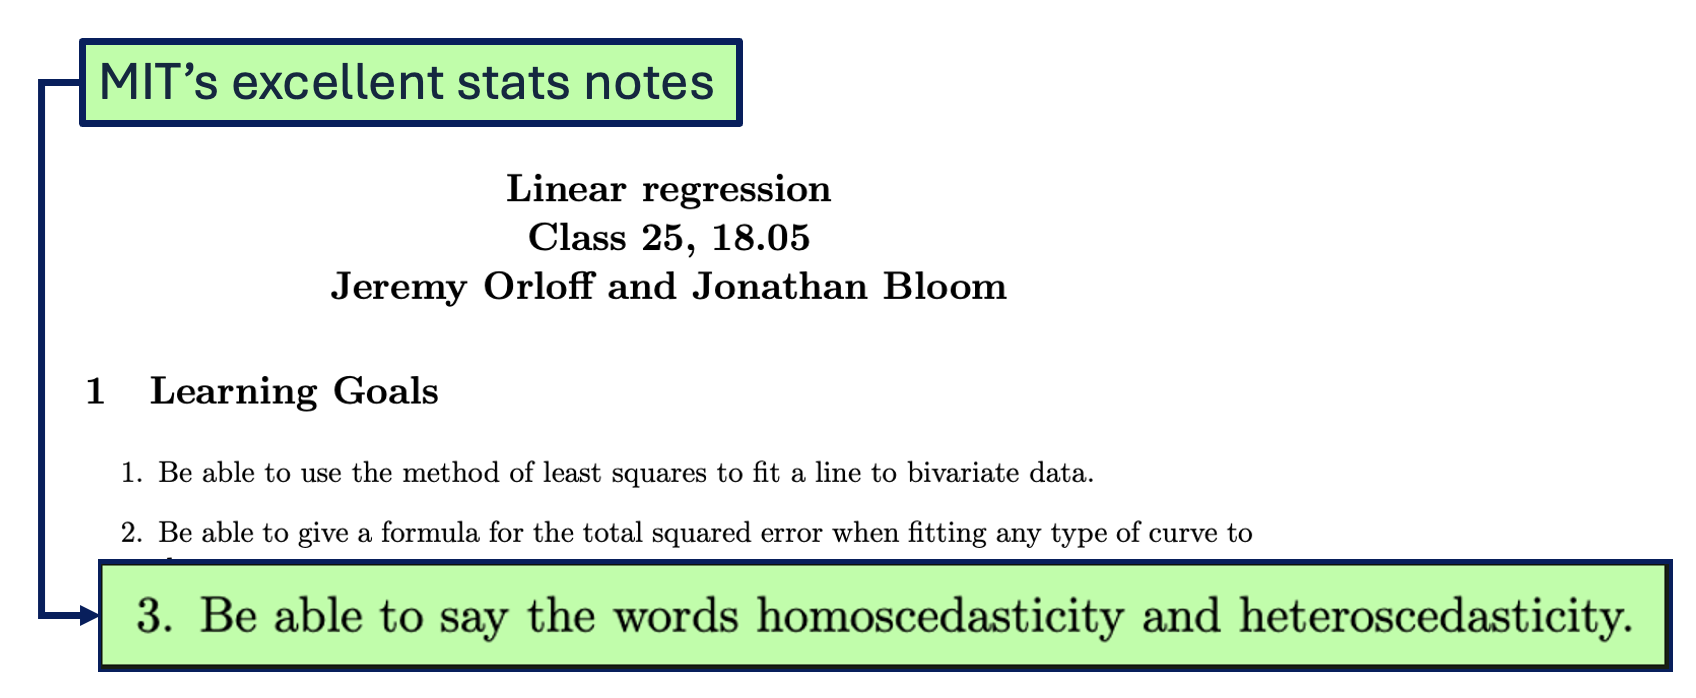
\includegraphics[scale=0.2]{mit-lol-1}
};
\end{tikzpicture}

\magtn{Ordinary Least Squares (OLS)}: For functions that are linear in their parameters. This does not mean they have to be linear in the RVs.\\[1ex]

\magtn{Nonlinear Least Squares (OLS)}: For functions that are nonlinear in their parameters.\\[1ex]

If the uncertainties on the measured data are \ghl{homoscedastic}, and serially uncorrelated (linearly), then the parameter estimates of OLS are the Minimum Variance Unbiased Estimates (MVUE - see Gauss-Markov theorem). \\[1ex]

If the data additionally have Gaussian uncertainties, then OLS and MLE are equivalent.\\[1ex]

\end{frame}

\begin{frame}{Variance of Residuals}
\footnotesize
For OLS to be the MVUE, the data should be Homoscedastic.\\[1ex]

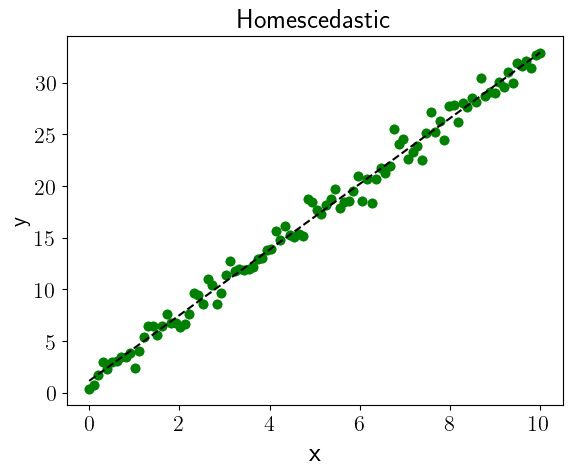
\includegraphics[scale=0.35]{Homo.png}
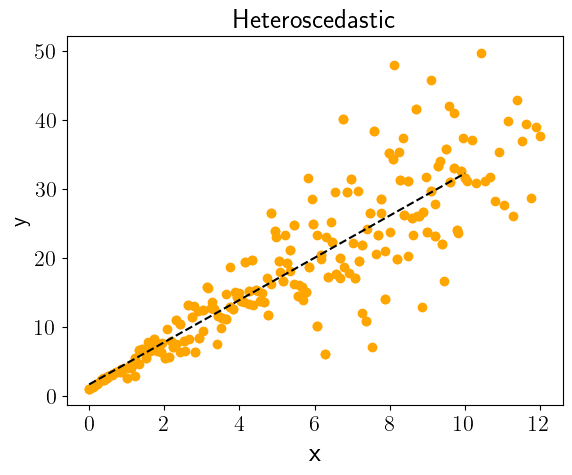
\includegraphics[scale=0.35]{Hetero.png}

If it is not, we can transform the data, or we can use Weighted LS (Like the Generalised LS example we went through, but with zero off-diagonal terms in the Cov matrix).
\end{frame}

\begin{frame}{Extreme Outliers }
\footnotesize
\begin{center}
\yhl{$\chi^2 = \sum\limits_i^N \dfrac{(y_i -\mu)^2 }{\sigma^2_i}$}
\end{center}

Squaring the residuals gives large weight to outliers: values of $y_i$ that deviate significantly from the best fit line that would result if they were excluded.\\[1ex]

\magtn{Robust Least Squares} refers to using a different statistic in the numerator (one that is less sensitive to outliers). \\[1ex]

One method for dealing with this is to use the Least Absolute Deviations method, which does not square the numerator.\\[1ex]

In \texttt{scipy.optimize.least\_squares}, this is controlled by specifying the \bbl{\texttt{loss}} argument - see workshop problems.

\end{frame}


\begin{frame}{Extreme Outliers}
\footnotesize
Example using \bbl{\texttt{loss=`soft\_l1', f\_scale=noise}} to ensure the outliers do not throw off the fit.

\begin{center}
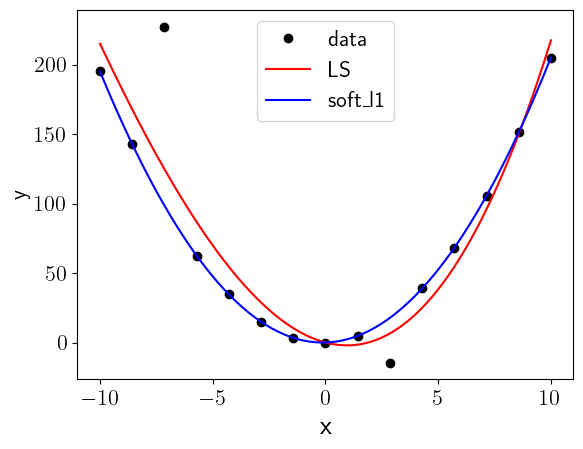
\includegraphics[scale=0.5]{robust-quadratic-ls.png}
\end{center}

\end{frame}




\begin{frame}{Other kinds of Regression}
\footnotesize
If the uncertainties on the data do not follow a normal distribution, we can use a Generalized Linear Model (GLM)- see python example with \texttt{statsmodels}. % In this example picture the `sideways' distributions in red indicate the data has a Poisson distribution on the right.\\[1ex]
\begin{center}
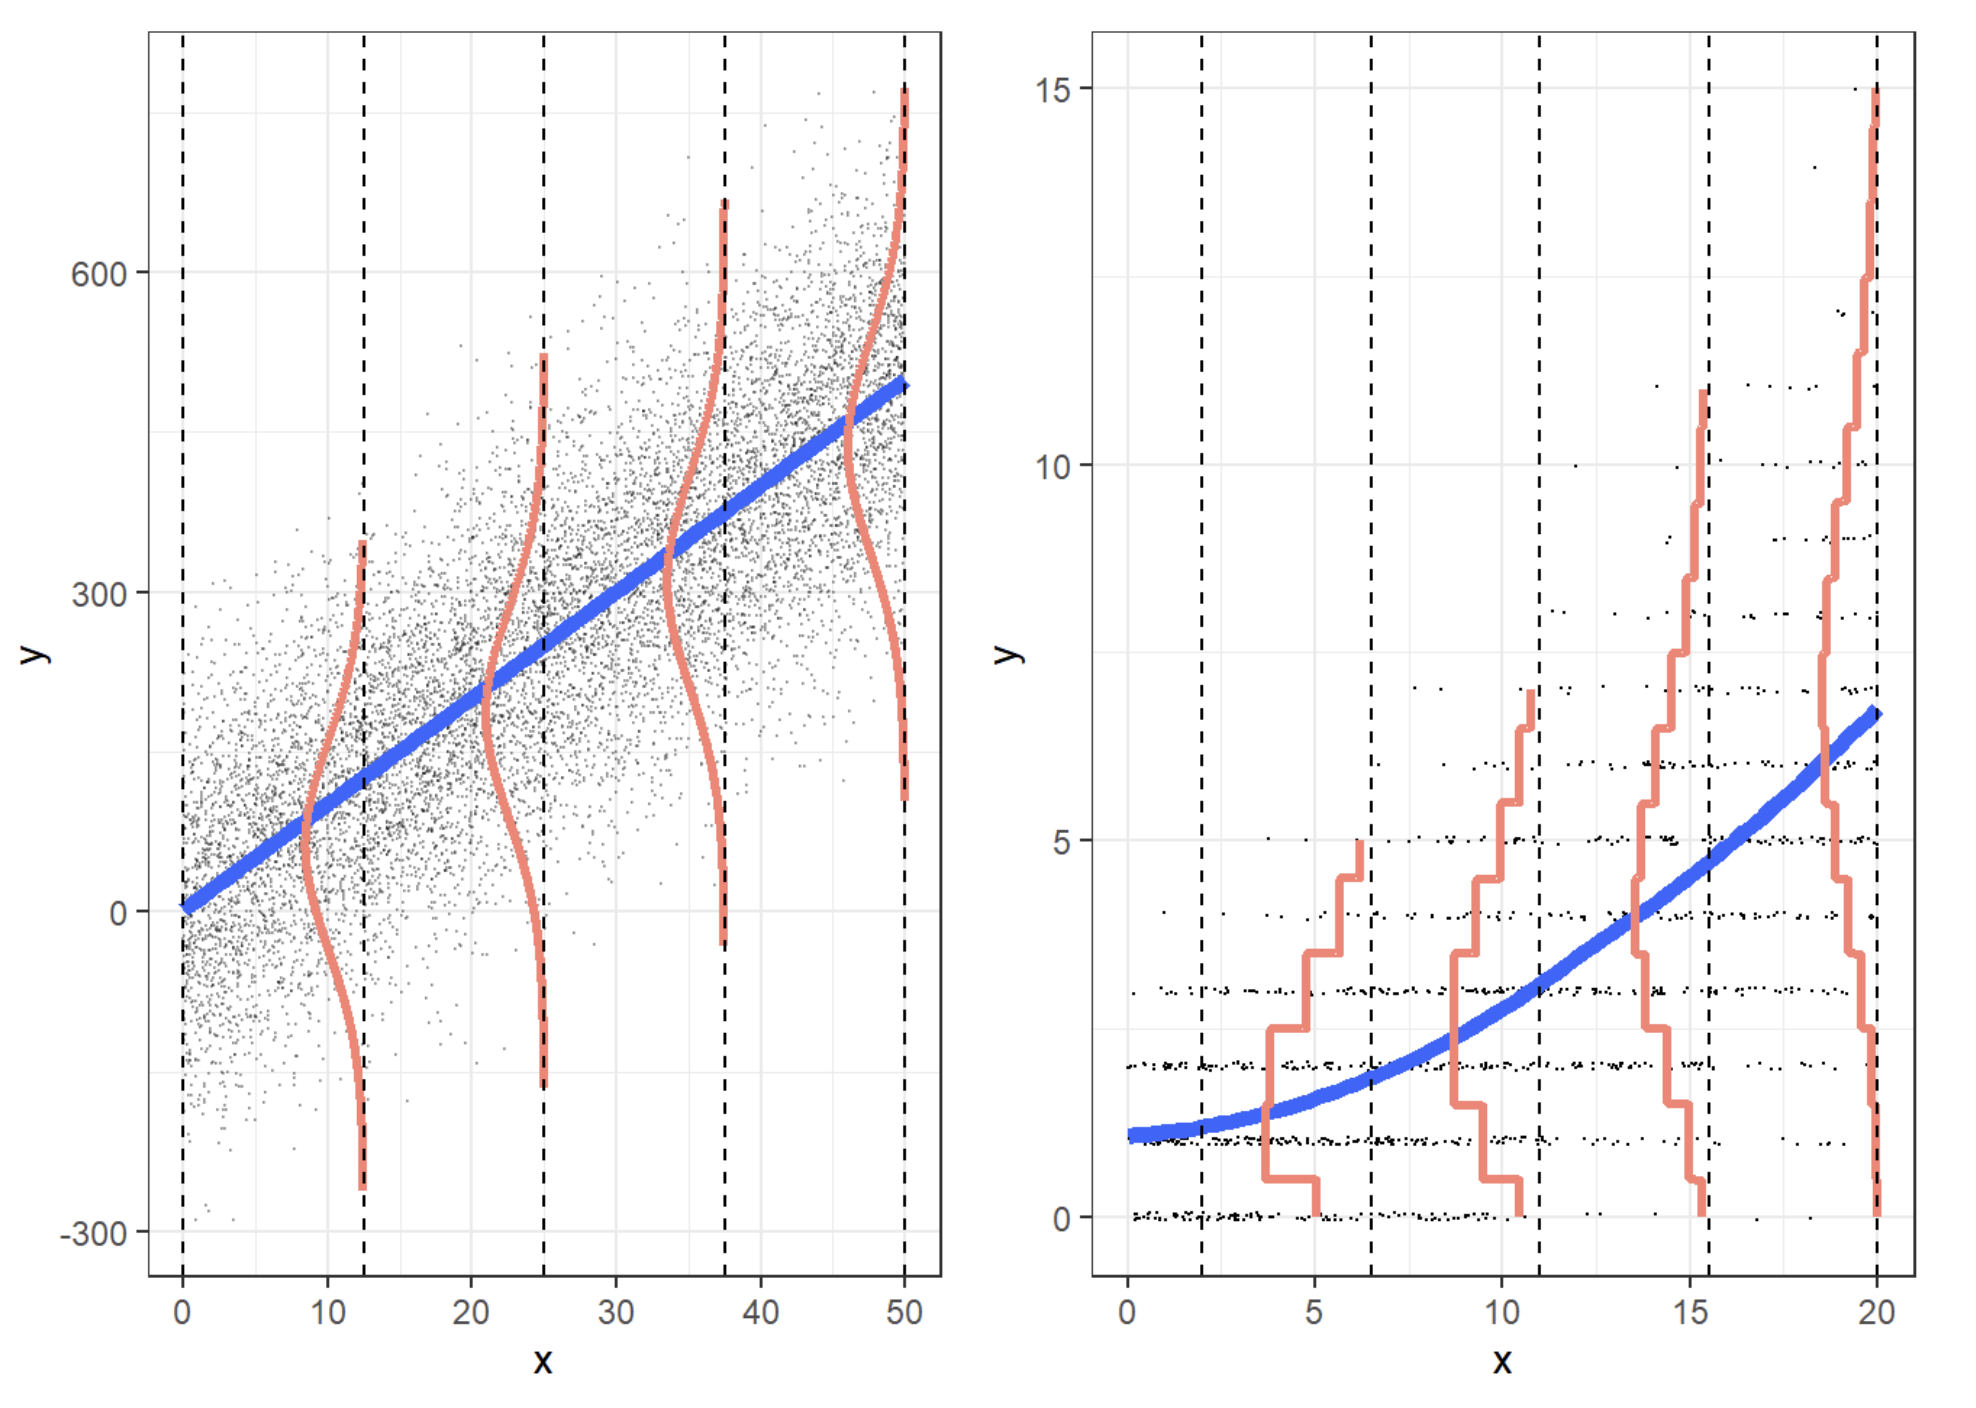
\includegraphics[scale=0.18]{PoissonRegression.png}

\tiny
PictureCredit: \href{https://bookdown.org/roback/bookdown-BeyondMLR/ch-poissonreg.html}{Roback \& Legler}\\ 
\end{center}
\end{frame}


%\begin{frame}{Binary Models}
%\footnotesize
%If the data is binary, for example pass/fail or true/false, you will probably use Logit or Probit Models.\\[1ex]
%
%Logit (\bbl{Log}istic un\bbl{it}) uses a logistic (aka sigmoid) CDF $F = [1 + \exp{ - (\theta_0 + \theta_1 x) }  ]^{-1}$\\[1ex]
%The argument of the exponential is a straight line with intercept $\theta_0 = \dfrac{-loc}{scale}$ and slope $\theta_1 = -\dfrac{1}{scale}$\\
%The Link Function is $\ln (\dfrac{p}{1-p}) $\\
%Probit (\bbl{Prob}ability un\bbl{it})  uses the normal CDF in its link function $F = \Phi(\theta_0 + \theta_1 x)$\\
%
%\end{frame}









\begin{frame}{Nonlinear Models}
\footnotesize
Functions that are not linear in the parameters, and cannot be linearised, can be solved iteratively rather than analytically. Methods for this include Simplex, and Gradient Search:\\[1ex]
\begin{enumerate}
\item Build a $N_p$-Dimensional parameter space such that each point in space is defined by a unique set of $\theta$.
\item First derivative $\grad_{\theta_j} \chi^2$ indicates sign and magntiude of slope.
\item Go downwards: we are seeking the minimum. $\theta_{j+1} = \theta_j - \gamma \grad_{\theta} \chi^2$\\[1ex]
\item Repeat.
\end{enumerate}
\vspace{0.5cm}

Things can go wrong with this, of course. Getting stuck in local minima, hyper focusing, and missing the turning points are all associated with choosing the step size $\gamma$ unwisely. Dark arts.

\end{frame}



\begin{frame}{Thanks For Your Time}
\center
\Huge
Fin.
\end{frame}

\end{document}







